\documentclass{standalone}
\usepackage{tikz}
\usepackage{verbatim}
\usetikzlibrary{positioning}
\begin{document}
\pagestyle{empty}
  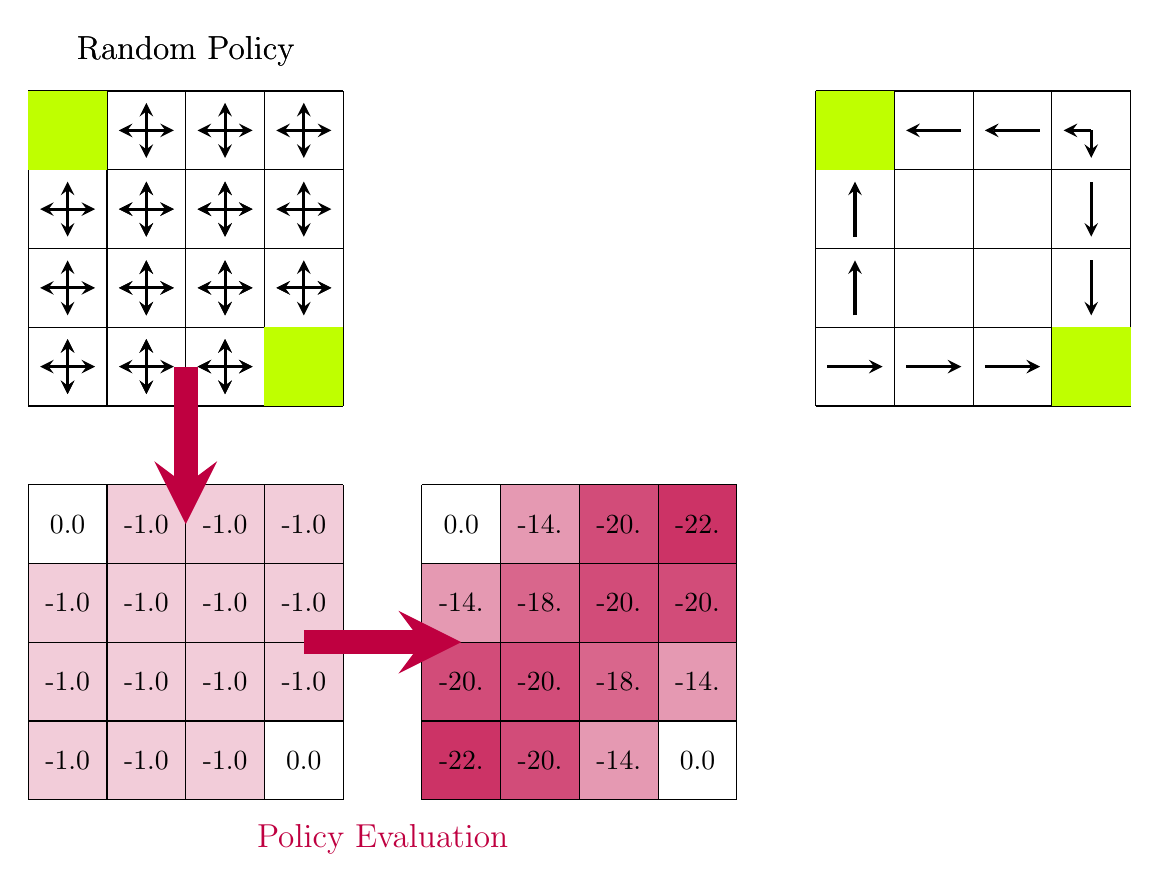
\begin{tikzpicture}

    \draw[step=1.0,black,thin] (0,0) grid (4, 4);
    \fill[lime] (0, 3) rectangle (1,4);
    \fill[lime] (3, 0) rectangle (4,1);
    % Top row.
    \draw[stealth-stealth, line width=0.4mm] (1.15, 3.5) -- (1.85, 3.5);
    \draw[stealth-stealth, line width=0.4mm] (1.5, 3.15) -- (1.5, 3.85);
    \draw[stealth-stealth, line width=0.4mm] (2.15, 3.5) -- (2.85, 3.5);
    \draw[stealth-stealth, line width=0.4mm] (2.5, 3.15) -- (2.5, 3.85);
    \draw[stealth-stealth, line width=0.4mm] (3.15, 3.5) -- (3.85, 3.5);
    \draw[stealth-stealth, line width=0.4mm] (3.5, 3.15) -- (3.5, 3.85);
    % Second from top row.
     \draw[stealth-stealth, line width=0.4mm] (0.15, 2.5) -- (0.85, 2.5);
    \draw[stealth-stealth, line width=0.4mm] (0.5, 2.15) -- (0.5, 2.85);
    \draw[stealth-stealth, line width=0.4mm] (1.15, 2.5) -- (1.85, 2.5);
    \draw[stealth-stealth, line width=0.4mm] (1.5, 2.15) -- (1.5, 2.85);
    \draw[stealth-stealth, line width=0.4mm] (2.15, 2.5) -- (2.85, 2.5);
    \draw[stealth-stealth, line width=0.4mm] (2.5, 2.15) -- (2.5, 2.85);
    \draw[stealth-stealth, line width=0.4mm] (3.15, 2.5) -- (3.85, 2.5);
    \draw[stealth-stealth, line width=0.4mm] (3.5, 2.15) -- (3.5, 2.85);
    % Second from bottom row.
    \draw[stealth-stealth, line width=0.4mm] (0.15, 1.5) -- (0.85, 1.5);
    \draw[stealth-stealth, line width=0.4mm] (0.5, 1.15) -- (0.5, 1.85);
    \draw[stealth-stealth, line width=0.4mm] (1.15, 1.5) -- (1.85, 1.5);
    \draw[stealth-stealth, line width=0.4mm] (1.5, 1.15) -- (1.5, 1.85);
    \draw[stealth-stealth, line width=0.4mm] (2.15, 1.5) -- (2.85, 1.5);
    \draw[stealth-stealth, line width=0.4mm] (2.5, 1.15) -- (2.5, 1.85);
    \draw[stealth-stealth, line width=0.4mm] (3.15, 1.5) -- (3.85, 1.5);
    \draw[stealth-stealth, line width=0.4mm] (3.5, 1.15) -- (3.5, 1.85);
    % Bottom row.
    \draw[stealth-stealth, line width=0.4mm] (1.15, 0.5) -- (1.85, 0.5);
    \draw[stealth-stealth, line width=0.4mm] (1.5, 0.15) -- (1.5, 0.85);
    \draw[stealth-stealth, line width=0.4mm] (2.15, 0.5) -- (2.85, 0.5);
    \draw[stealth-stealth, line width=0.4mm] (2.5, 0.15) -- (2.5, 0.85);
    \draw[stealth-stealth, line width=0.4mm] (0.15, 0.5) -- (0.85, 0.5);
    \draw[stealth-stealth, line width=0.4mm] (0.5, 0.15) -- (0.5, 0.85);
    \node at (2, 4.5) {\large Random Policy};

    \node at (0.5, -1.5) {0.0};
    \fill[purple!20] (1, -2) rectangle (2,-1);
    \node at (1.5, -1.5) {-1.0};
    \fill[purple!20] (2, -2) rectangle (3,-1);
    \node at (2.5, -1.5) {-1.0};
    \fill[purple!20] (3, -2) rectangle (4,-1);
    \node at (3.5, -1.5) {-1.0};
    % Second frop top row.
    \fill[purple!20] (0, -3) rectangle (1,-2);
    \node at (0.5, -2.5) {-1.0};
    \fill[purple!20] (1, -3) rectangle (2,-2);
    \node at (1.5, -2.5) {-1.0};
    \fill[purple!20] (2, -3) rectangle (3,-2);
    \node at (2.5, -2.5) {-1.0};
    \fill[purple!20] (3, -3) rectangle (4,-2);
    \node at (3.5, -2.5) {-1.0};
    % Second from bottom row.
    \fill[purple!20] (0, -4) rectangle (1,-3);
    \node at (0.5, -3.5) {-1.0};
    \fill[purple!20] (1, -4) rectangle (2,-3);
    \node at (1.5, -3.5) {-1.0};
    \fill[purple!20] (2, -4) rectangle (3,-3);
    \node at (2.5, -3.5) {-1.0};
    \fill[purple!20] (3, -4) rectangle (4,-3);
    \node at (3.5, -3.5) {-1.0};
    % Bottom row.
    \fill[purple!20] (0, -5) rectangle (1,-4);
    \node at (0.5, -4.5) {-1.0};
    \fill[purple!20] (1, -5) rectangle (2,-4);
    \node at (1.5, -4.5) {-1.0};
    \fill[purple!20] (2, -5) rectangle (3,-4);
    \node at (2.5, -4.5) {-1.0};
    \node at (3.5, -4.5) {0.0};
    \draw[step=1.0,black] (0,-5) grid (4, -1);
    \draw[-stealth, line width=3mm, purple] (2, 0.5) -- (2, -1.5);

    \node at (5.5, -1.5) {0.0};
    \fill[purple!40] (6, -2) rectangle (7,-1);
    \node at (6.5, -1.5) {-14.};
    \fill[purple!70] (7, -2) rectangle (8,-1);
    \node at (7.5, -1.5) {-20.};
    \fill[purple!80] (8, -2) rectangle (9,-1);
    \node at (8.5, -1.5) {-22.};
    % Second frop top row.
    \fill[purple!40] (5, -3) rectangle (6,-2);
    \node at (5.5, -2.5) {-14.};
    \fill[purple!60] (6, -3) rectangle (7,-2);
    \node at (6.5, -2.5) {-18.};
    \fill[purple!70] (7, -3) rectangle (8,-2);
    \node at (7.5, -2.5) {-20.};
    \fill[purple!70] (8, -3) rectangle (9,-2);
    \node at (8.5, -2.5) {-20.};
    % Second from bottom row.
    \fill[purple!70] (5, -4) rectangle (6,-3);
    \node at (5.5, -3.5) {-20.};
    \fill[purple!70] (6, -4) rectangle (7,-3);
    \node at (6.5, -3.5) {-20.};
    \fill[purple!60] (7, -4) rectangle (8,-3);
    \node at (7.5, -3.5) {-18.};
    \fill[purple!40] (8, -4) rectangle (9,-3);
    \node at (8.5, -3.5) {-14.};
    % Bottom row.
    \fill[purple!80] (5, -5) rectangle (6,-4);
    \node at (5.5, -4.5) {-22.};
    \fill[purple!70] (6, -5) rectangle (7,-4);
    \node at (6.5, -4.5) {-20.};
    \fill[purple!40] (7, -5) rectangle (8,-4);
    \node at (7.5, -4.5) {-14.};
    \node at (8.5, -4.5) {0.0};
    \draw[step=1.0,black] (5,-5) grid (9, -1);
    \draw[-stealth, line width=3mm, purple] (3.5, -3) -- (5.5, -3);
    \node [text=purple] at (4.5, -5.5) {\large Policy Evaluation};

    \draw[step=1.0,black,thin] (10,0) grid (14, 4);
    \fill[lime] (10, 3) rectangle (11,4);
    \fill[lime] (13, 0) rectangle (14,1);
    % Top row.
    \draw[stealth-, line width=0.4mm] (11.15, 3.5) -- (11.85, 3.5);
    \draw[stealth-, line width=0.4mm] (12.15, 3.5) -- (12.85, 3.5);
    \draw[-stealth, line width=0.4mm] (13.5, 3.5) -- (13.15, 3.5);
    \draw[-stealth, line width=0.4mm] (13.5, 3.5) -- (13.5, 3.15);
    % Second from top row.
    \draw[-stealth, line width=0.4mm] (10.5, 2.15) -- (10.5, 2.85);
    \draw[stealth-stealth, line width=0.4mm] (1.15, 2.5) -- (1.85, 2.5);
    \draw[stealth-stealth, line width=0.4mm] (1.5, 2.15) -- (1.5, 2.85);
    \draw[stealth-stealth, line width=0.4mm] (2.15, 2.5) -- (2.85, 2.5);
    \draw[stealth-stealth, line width=0.4mm] (2.5, 2.15) -- (2.5, 2.85);
    \draw[stealth-, line width=0.4mm] (13.5, 2.15) -- (13.5, 2.85);
    % Second from bottom row.
    \draw[-stealth, line width=0.4mm] (10.5, 1.15) -- (10.5, 1.85);
    \draw[stealth-stealth, line width=0.4mm] (1.15, 1.5) -- (1.85, 1.5);
    \draw[stealth-stealth, line width=0.4mm] (1.5, 1.15) -- (1.5, 1.85);
    \draw[stealth-stealth, line width=0.4mm] (2.15, 1.5) -- (2.85, 1.5);
    \draw[stealth-stealth, line width=0.4mm] (2.5, 1.15) -- (2.5, 1.85);
    \draw[stealth-stealth, line width=0.4mm] (3.15, 1.5) -- (3.85, 1.5);
    \draw[stealth-, line width=0.4mm] (13.5, 1.15) -- (13.5, 1.85);
    % Bottom row.
    \draw[-stealth, line width=0.4mm] (11.15, 0.5) -- (11.85, 0.5);
    \draw[-stealth, line width=0.4mm] (12.15, 0.5) -- (12.85, 0.5);
    \draw[stealth-stealth, line width=0.4mm] (1.5, 0.15) -- (1.5, 0.85);
    \draw[stealth-stealth, line width=0.4mm] (2.15, 0.5) -- (2.85, 0.5);
    \draw[stealth-stealth, line width=0.4mm] (2.5, 0.15) -- (2.5, 0.85);
    \draw[-stealth, line width=0.4mm] (10.15, 0.5) -- (10.85, 0.5);
    \draw[stealth-stealth, line width=0.4mm] (0.5, 0.15) -- (0.5, 0.85);
    \node at (2, 4.5) {\large Random Policy};

  \end{tikzpicture}
\end{document}